\newpage
\section*{{\Large 문제 E.} \tabto{2cm}{\LARGE 숫자탑과 쿼리}}

\begin{itemize}
    \item 시간 제한 \tabto{2cm} 2초
\end{itemize}

\hrule

\subsection*{문제}

의찬이는 숫자가 적힌 블록으로 탑 쌓기를 즐긴다. 어느 날 선우는 의찬이가 쌓는 탑에 규칙이 있음을 알게 되었다! 선우가 알아낸 규칙은 다음과 같다.

\begin{itemize}
    \item 의찬이가 쌓는 탑은 꼭대기가 $1$층이고, $1$층에는 $a$개의 블록이 존재한다.
    \item $1$층의 가장 왼쪽 블록에는 $1$이 적혀있으며, 블록에 적힌 숫자는 오른쪽으로 갈수록 $1$씩 증가한다.
    \item $i$번째 층의 가장 오른쪽 블록보다 $i+1$번째 층의 가장 왼쪽 블록이 $1$더 크다.
    \item $i$번째 층에 있는 블록의 수보다 $i+1$번째 층에 있는 블록의 수가 $d$개 더 많다.
\end{itemize}

아래 그림은 $1$에서 $4$층까지 $a=1$이고 $d=2$일 때 의찬이가 쌓은 탑의 모습이다.

\begin{figure}[h]
    \centering
    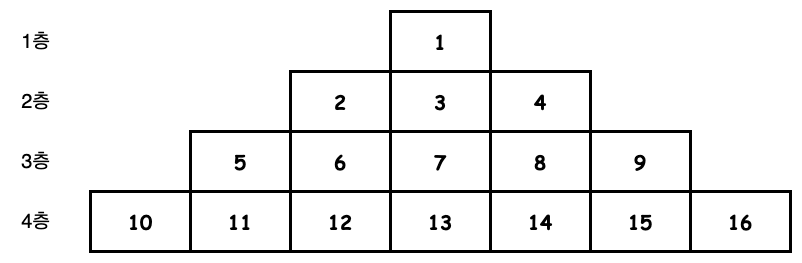
\includegraphics[width=0.6\textwidth]{problems/image/sootab.png}
    % \caption{[그림 1]}
\end{figure}

각 숫자가 적힌 블록의 위치를 모조리 외운 의찬이는 선우가 던지는 $Q$개의 질문에 답하고자 한다. 질문은 한 가지 형식이다.

\begin{itemize}
    \item \texttt{\color{red}a d x} : $a$와 $d$가 주어질 때, $x$가 적힌 숫자 블록이 몇 번째 층의 몇 번째 숫자인가?
\end{itemize}

위 그림을 예로 들자. 만약 $a=1$, $d=2$, $x=12$라면 의찬이는 $(4,3)$이라고 대답한다. 이는 $12$가 적힌 숫자 블록이 $4$층에 위치한 $3$번째 숫자라는 것을 의미한다.

\subsection*{입력}

첫째 줄에는 선우가 의찬이에게 하는 질문의 개수 $Q$가 주어진다. $(1\leq Q \leq 500\,000)$

이후 $Q$개의 줄에는 $a$, $d$, $x$가 공백으로 구분되어 주어진다. $(1\leq a,d,x \leq 10^{6})$

입력으로 주어지는 모든 값은 정수다.

\subsection*{출력}

$Q$개의 줄에 걸쳐 $x$번째 블록이 위치한 층과 가장 왼쪽을 기준으로 몇 번째 칸에 위치하는지 출력하시오.

\newpage

\subsection*{예제}

\begin{table}[h]
% \centering
\renewcommand{\arraystretch}{1.5}
\begin{tabular}{|L{8.2cm}|L{8.2cm}|}
\hline
\multicolumn{1}{|c|}{\textbf{standard input}} & \multicolumn{1}{c|}{\textbf{standard output}} \\ \hline\hline
% 적절한 예제를 입력하면 됩니다.
\texttt{2} & \texttt{4 3}\\ 
\texttt{1 2 12} & \texttt{5 1}\\
\texttt{1 2 17} & \\

\hline
\end{tabular}
\end{table}